% Options for packages loaded elsewhere
\PassOptionsToPackage{unicode}{hyperref}
\PassOptionsToPackage{hyphens}{url}
%
\documentclass[
]{article}
\usepackage{lmodern}
\usepackage{amssymb,amsmath}
\usepackage{ifxetex,ifluatex}
\ifnum 0\ifxetex 1\fi\ifluatex 1\fi=0 % if pdftex
  \usepackage[T1]{fontenc}
  \usepackage[utf8]{inputenc}
  \usepackage{textcomp} % provide euro and other symbols
\else % if luatex or xetex
  \usepackage{unicode-math}
  \defaultfontfeatures{Scale=MatchLowercase}
  \defaultfontfeatures[\rmfamily]{Ligatures=TeX,Scale=1}
\fi
% Use upquote if available, for straight quotes in verbatim environments
\IfFileExists{upquote.sty}{\usepackage{upquote}}{}
\IfFileExists{microtype.sty}{% use microtype if available
  \usepackage[]{microtype}
  \UseMicrotypeSet[protrusion]{basicmath} % disable protrusion for tt fonts
}{}
\makeatletter
\@ifundefined{KOMAClassName}{% if non-KOMA class
  \IfFileExists{parskip.sty}{%
    \usepackage{parskip}
  }{% else
    \setlength{\parindent}{0pt}
    \setlength{\parskip}{6pt plus 2pt minus 1pt}}
}{% if KOMA class
  \KOMAoptions{parskip=half}}
\makeatother
\usepackage{xcolor}
\IfFileExists{xurl.sty}{\usepackage{xurl}}{} % add URL line breaks if available
\IfFileExists{bookmark.sty}{\usepackage{bookmark}}{\usepackage{hyperref}}
\hypersetup{
  pdftitle={Final project},
  pdfauthor={Laura Conover},
  hidelinks,
  pdfcreator={LaTeX via pandoc}}
\urlstyle{same} % disable monospaced font for URLs
\usepackage[margin=1in]{geometry}
\usepackage{graphicx,grffile}
\makeatletter
\def\maxwidth{\ifdim\Gin@nat@width>\linewidth\linewidth\else\Gin@nat@width\fi}
\def\maxheight{\ifdim\Gin@nat@height>\textheight\textheight\else\Gin@nat@height\fi}
\makeatother
% Scale images if necessary, so that they will not overflow the page
% margins by default, and it is still possible to overwrite the defaults
% using explicit options in \includegraphics[width, height, ...]{}
\setkeys{Gin}{width=\maxwidth,height=\maxheight,keepaspectratio}
% Set default figure placement to htbp
\makeatletter
\def\fps@figure{htbp}
\makeatother
\setlength{\emergencystretch}{3em} % prevent overfull lines
\providecommand{\tightlist}{%
  \setlength{\itemsep}{0pt}\setlength{\parskip}{0pt}}
\setcounter{secnumdepth}{-\maxdimen} % remove section numbering

\title{Final project}
\author{Laura Conover}
\date{}

\begin{document}
\maketitle

\hypertarget{abstract}{%
\section{Abstract}\label{abstract}}

Human speech sounds are full of variation. Some of this variation is
phonemic - to English speakers, the difference between the unvoiced `p'
sound in `pug' and the voiced `b' sound in `bug' completely changes the
meaning of the resulting word. On the other hand, not all variation
within speech sounds carry meaning, such as the contrast between the
aspirated `p' sound in `pot' and the unaspirated `p' sound in `spot' for
English speakers. Although the type of contrast that is considered
important varies between languages (aspiration contrasts are meaningful
in languages such as Hindu, Thai, and Punjabi), it is a general rule
that adults have a difficult time perceiving non-phonemic contrasts. It
is possible, however, that certain acoustic markers may interact with
individual listener characteristics to make some non-phonemic contrasts
more easily perceptible for some listeners than others. The following
study examines such interactions, with the results implying that (XYZ,
whatever the ACTUAL study shows but I really hope it's in line with
Kuhl's Perceptual Magnets otherwise I've got issues).

\hypertarget{acknowledgements}{%
\section{Acknowledgements}\label{acknowledgements}}

Much thanks to Richard Layton for his
tutorial{[}\url{https://rmarkdown.rstudio.com/articles_docx.html}{]} on
a work-around for formatting when the \texttt{papaja} package was too
frustrating.

\hypertarget{introduction-and-disclaimer}{%
\section{Introduction (and
disclaimer)}\label{introduction-and-disclaimer}}

The data selected comes from a study of individuals' perceptions of both
spontaneous and volitional laughter produced by young adult female
American English speakers. The discrepency between this description and
what was mentioned in the abstract is obvious. Clearly, this is not at
all the data set that will be used in the final study. However, the
structure of the data and variables are identical to the structure of
the study's data: responses to a 2A-FC test, categorical listener
variables, and continuous acoustic variables. Therefore, this data is a
good stand-in until actual data collection is complete. Similarly, not
all of the descriptive text is finalized. I hope that what is written
here and in the folder's README file will provide sufficient
explanation.

\hypertarget{methods}{%
\section{Methods}\label{methods}}

The original data includes two csv files: one detailing information on
the acoustic features of the laugh stimuli (including
spontaneous/volitional condition and duration, voicing, pitch, and
intensity measures), and the other detailing information on the
listeners and perceptions (including basic demographic data such as
gender, country of origin, English fluency, and education, as well as
whether each stimulus was perceived as volitional or spontaneous). This
dataset has no missing values; it is possible that any cases with
missing values were deleted listwise prior to publication. Even so,
these data files are somewhat messy. Participant IDs were reused at
different sites, and stimulus files were renamed between analyses.
Additionally, there are a number of variables that are not relevant to
the current project. As such, the data were slightly cleaned and
reorganized prior to analysis.

Selected variables for this analysis include: Laugh condition
(spontaneous or volitional), accuracy of listener's judgement on a
trial, total laugh duration in seconds, the average pitch of the laugh
in logHz, and the listener's country of origin.

\hypertarget{data-analysis}{%
\subsection{Data analysis}\label{data-analysis}}

The average accuracy by listener's country of origin is presented in
Table 1 below. Although the scores do vary from country to country, the
range of scores only reaches from 0.5621693 to 0.6856725, with an
average accuracy of 0.6371769.

(Insert some transition here from visual analysis of listener
characteristics to visual analysis of stimulus characteristics depending
on actual data.)

The influence of acoustic features on hit rates - or, rather, the
apparent lack thereof - can be seen in Figure one:

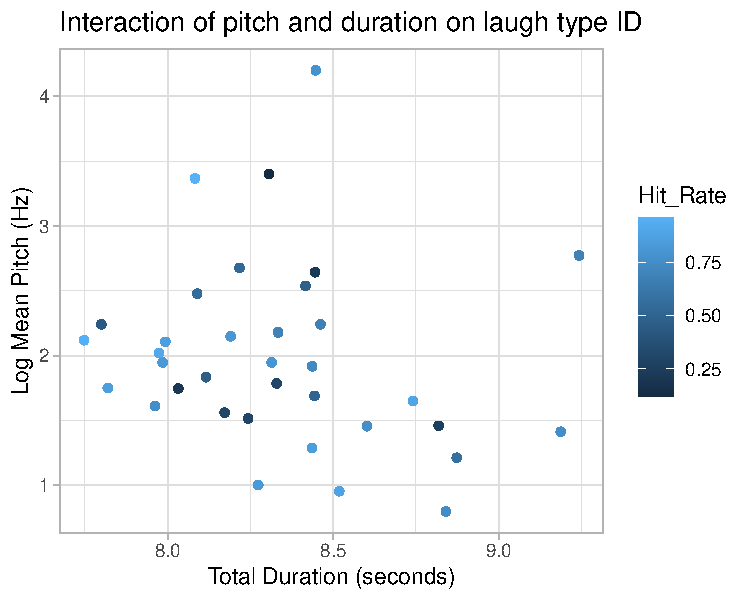
\includegraphics{C:/Users/Me/Desktop/data science/DataSci-hw-lconover1/final_project/output/pdf_document/final_files/figure-latex/unnamed-chunk-2-1.pdf}

(Insert a lovely transition about the usefulness of models, part of my
committee is pushing towards single-subject designs by requesting
visualizations first and that's not what I'm doing but ok.)

Note that, in Table 2 below, there is no significant difference in
either pitch or duration, or their interaction, between the two stimulus
conditions. That is, there is no acoustic difference between spontaneous
and volitional laughter within these two measures. (A statement I better
be able to change for my actual data.)

However, the human perceptual system is modified by more factors than
just acoustic information. As seen in Table 3 below, the listener's
country of origin does impact whether or not the listener can correctly
perceive a stimulus as spontaneous or volitional, \(R^2 = .19\),
\(F(20, 863) = 10.24\), \(p < .001\)

(Yes, I understand that's not EXACTLY what these variables mean in the
given dataset and that I'm talking about two different things, but the
process of getting there is closest to what I'll eventually be doing.
Although there are a heck of a lot more countries than there will be
conditions for what I'm doing.)

\end{document}
